\chapter{Syntax parameters}
\textcolor{white}{``}
Syntax parameter are a mechanism for rebinding a macro definition within the dynamic extent of a macro expansion. With syntax parameters instead of introducing the unhygienic binding each time we instead create a binding for the keyword, which we can adjust later when we want the keyword to have a different meaning. As no new binding is introduced so hygiene is preserved, This is similar to the dynamic binding mechanism that we have at run time, except that the dynamic binding only occurs during macro expansion.
\textcolor{white}{''}
\section{Pre-processing [Approach 1]}
\textcolor{white}{``}
In this approach I tried to use pre-processing approach similar to C, where I transform the code before the main compiler gets hold of it. \texttt{``SyntaxParameter"} replaces and binds the parameter with its mapped value in the particular defined macro scope. Here the macro transformation happens during the parse phase by matching the pattern. To define syntax parameters in Sweet.JS, the programmer provides a new keyword that looks something like this:  
\textcolor{white}{''}
\begin{lstlisting}[frame=single]
SyntaxParameter(<parameter>,<Mapped to>,
<Scope/Macro Name>,<Macro definition>)
\end{lstlisting}

``parameter" an identifier that is defined as a syntax parameter in the macro definition, \textit{``Mapped to"} is the macro input variable that will be mapped to \textit{``parameter,"} \textit{``Scope'} define the context of the macro definition.
\newpage
An example of its usage is Figure 8:

\begin{figure}[htb]
\centering
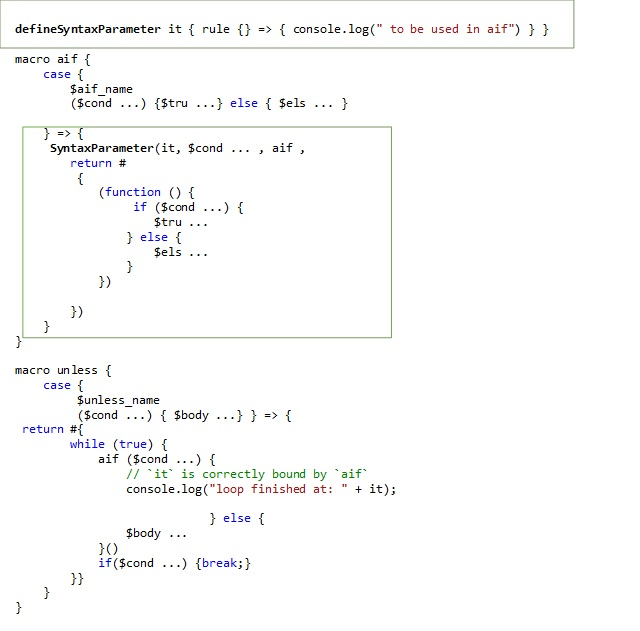
\includegraphics[width=1.0\textwidth]{images/Appraoch1.jpg}
\caption{Approach 1.} 
\label{fig:AST1}
\end{figure}
\begin{figure}[htb]
\centering
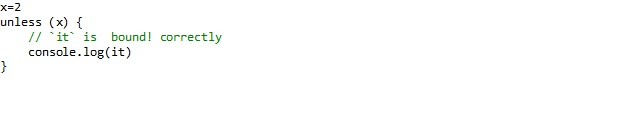
\includegraphics[width=1.0\textwidth]{images/Appraoch2.jpg}
\caption{Calling unless macro} 
\label{fig:AST2}

\end{figure}

The expanded code looks like:

\begin{figure}[htb]
\centering
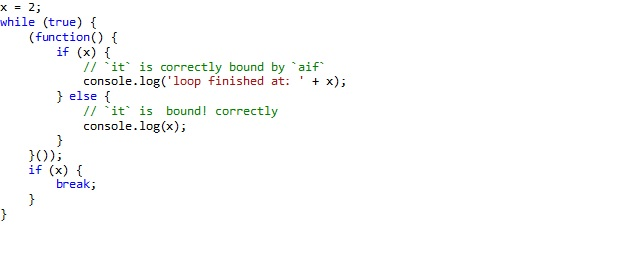
\includegraphics[width=1.0\textwidth]{images/Appraoch3.jpg}
\caption{ it identifier is correctly bounded to \$cond.. Of an anaphoric-if} 
\label{fig:AST3}

\end{figure}

As the example in Figure 10 shows, \texttt{`it'} is correctly bounded to \$cond.. as desired, However this approach has certain disadvantages, since this won`t allow users to define macros named \texttt{``SyntaxParameter''} 
\textcolor{white}{``}
At the moment in Sweet.JS the only way to create a syntax transformer is by defining a macro. A macro is really just a function that takes syntax and returns syntax (thus a syntax transformer). To fix this we first need to implement some primitive function that help us to create and manipulate the arbitrary compile time syntax transformation. Macros are compile time syntax transformation, so when the ``expander'' encounters a macro definition, it converts the body of the macro into a function and loads it into the compile time environment.
\textcolor{white}{''}
\newpage
\section{Syntax parameter processing at compile time [Approach 2]}
\textcolor{white}{``}
In this approach I defined ``syntaxparam'' similar to define-syntax-parameter in Scheme, which loads the primitive function in compile time environment,''syntaxLocalValue,'' which load the compile time primitive function from the environment and ``replaceSyntaxParam,'' which transforms the identifier with the compile time value from the environment returned by ''syntaxLocalValue,''  within the defined scope of the macro. Example shown below
\textcolor{white}{''}
\begin{figure}[htb]
\centering
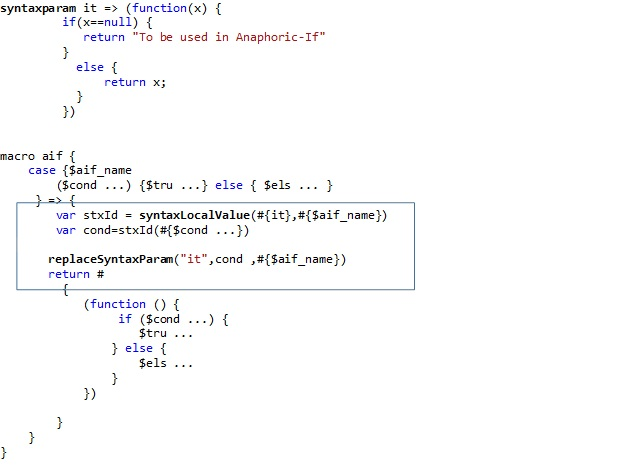
\includegraphics[width=1.0\textwidth]{images/Appraoch21.jpg}

\label{fig:AST4}
\end{figure}
\newpage
\begin{figure}[htb]
\centering
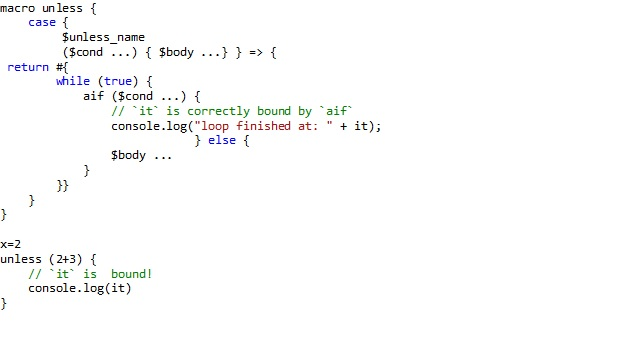
\includegraphics[width=1.0\textwidth]{images/Appraoch23.jpg}
\caption{ Approach 2.Syntax parameter implementation contd..} 
\label{fig:AST5}
\end{figure}

In Figure 11, i have defined an anaphoric-if macro named as \textit{aif}, where \textit{syntaxLocalValue} define an identifier \textit{it} as a syntax parameter defined in the \textit{aif} macro context, which also load the macro definition for \textit{it} from the context environment. Once the macro definition is loaded, then \textit{replaceSyntaxParam} replace the identifier with the defined identifier definition during expansion of the macro.
 
\begin{figure}[htb]
\centering
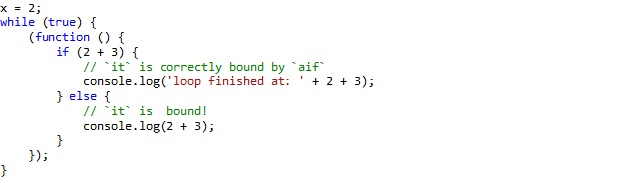
\includegraphics[width=1.0\textwidth]{images/Appraoch22.jpg}
\caption{ Approach 2. Syntax parameter expansion} 
\label{fig:AST6}
\end{figure}

Figure 12, show the expanded result of the ``unless'' macro defined in Figure 11, and it expand as expected.

\newpage
\begin{figure}[htb]
\centering
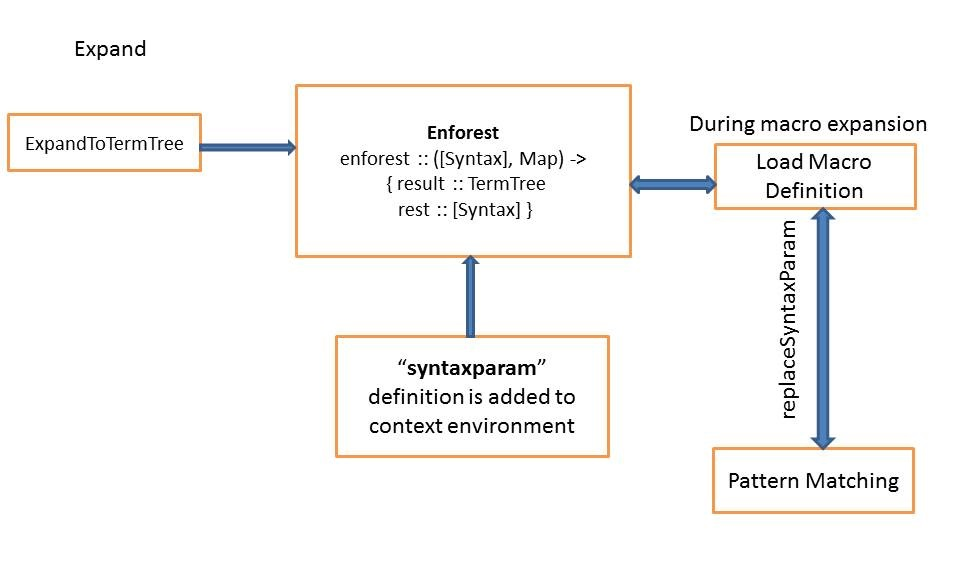
\includegraphics[width=1.0\textwidth]{images/CodeWorking.jpg}
\caption{ Approach 2. Implementation } 
\label{fig:AST7}
\end{figure}

The main entry point into the expander is, expand function is primarily responsible for handling hygiene. The \texttt{env} param is a mapping from identifier to macro definitions and \texttt{ctx} is a mapping of names to names. The expand function delegates to expandToTermTree, responsible for converting the syntax to TermTrees and loading any macro definitions it finds into the new env map.

Its in the ``expandToTermTree,'' it call enforest repeatedly until the entire token tree has been converted into a term tree. its in enforest function where ``syntaxparam'' definition loaded to context env map. When macro call is invoked it load the macro definition from the env in ``loadmacrodef'' function and during pattern matching ``replaceSyntaxParam'' which, bind the identifier with the value.
